\documentclass[tikz,border=5pt]{standalone}
\usepackage{tikz}
\definecolor{blueC}{RGB}{30,90,220}
\definecolor{purpC}{RGB}{125,40,170}
\definecolor{greenC}{RGB}{0,140,60}
\definecolor{orangeC}{RGB}{255,140,40}

\usetikzlibrary {arrows.meta}

\begin{document}
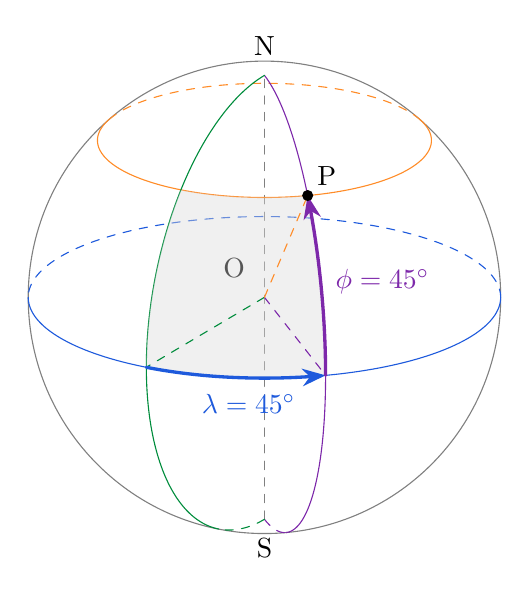
\begin{tikzpicture}[line cap=round, line join=round]

% ================= Panel 1: orthographic 3D view =================
% View tilt 20 deg, globe rotated 30 deg about the polar axis
\node[label=above:N]      (nord)   at (0, 2.819) {};
\node[label=above left:O] (centre) at (0, 0) {};
\node[label=below:S]      (sud)    at (0, -2.819) {};

\draw[gray] (centre) circle (3);
\draw[gray, thin, dashed] (sud.center) -- (nord.center);

% Equator: front solid, back dashed
\draw[blueC, thin] plot[domain=-60:120,samples=120]
  ({3*sin(\x-30)}, {-1.026*cos(\x-30)});
\draw[blueC, thin, dashed] plot[domain=120:300,samples=120]
  ({3*sin(\x-30)}, {-1.026*cos(\x-30)});

% 45 N parallel: front solid, back dashed
\draw[orangeC, thin] plot[domain=-81.35:141.35,samples=150]
  ({2.121*sin(\x-30)}, {2.121*(0.9397-0.342*cos(\x-30))});
\draw[orangeC, thin, dashed] plot[domain=141.35:278.65,samples=150]
  ({2.121*sin(\x-30)}, {2.121*(0.9397-0.342*cos(\x-30))});

% 45 E meridian: front solid, back dashed
\draw[purpC, thin] plot[domain=-69.4:90,samples=120]
  ({0.7765*cos(\x)}, {2.819*sin(\x)-0.991*cos(\x)});
\draw[purpC, thin, dashed] plot[domain=-90:-69.4,samples=40]
  ({0.7765*cos(\x)}, {2.819*sin(\x)-0.991*cos(\x)});

% Greenwich meridian: curved in 3D, front solid, back dashed
\draw[greenC, thin] plot[domain=-67.2:90,samples=120]
  ({-1.5*cos(\x)}, {2.819*sin(\x)-0.888*cos(\x)});
\draw[greenC, thin, dashed] plot[domain=-90:-67.2,samples=40]
  ({-1.5*cos(\x)}, {2.819*sin(\x)-0.888*cos(\x)});

% Curved patch 30-60 E, 30-60 N
\fill[black!15, opacity=0.4]
     plot[domain=0:45,samples=40] ({3*sin(\x-30)}, {-1.026*cos(\x-30)})
  -- plot[domain=0:45,samples=40] ({0.7765*cos(\x)}, {2.819*sin(\x)-0.991*cos(\x)})
  -- plot[domain=0:45,samples=40] ({-1.5*cos(\x)}, {2.819*sin(\x)-0.888*cos(\x)})
  -- plot[domain=0:45,samples=40] ({2.121*sin(\x-30)}, {2.121*(0.9397-0.342*cos(\x-30))})
  -- cycle;

% Rays from the centre
\draw[greenC, thin, dashed]  (0,0) -- (-1.5,-0.888);
\draw[purpC, thin, dashed]   (0,0) -- (0.777,-0.991);
\draw[orangeC, thin, dashed] (0,0) -- (0.549,1.293);

% Measured lambda arc (equator, Greenwich to 45 E) and phi arc (equator to P)
\draw[blueC, very thick, -Stealth] plot[domain=0:45,samples=40]
  ({3*sin(\x-30)}, {-1.026*cos(\x-30)});
\draw[purpC, very thick, -Stealth] plot[domain=0:45,samples=40]
  ({0.7765*cos(\x)}, {2.819*sin(\x)-0.991*cos(\x)});

% Point P (45 N, 45 E)
\fill (0.549,1.293) circle (2pt) node[above right] {P};
\node[blueC] at (-0.2,-1.35) {$\lambda=45^\circ$};
\node[purpC] at (1.5,0.2) {$\phi=45^\circ$};
%\node at (0,-3.6) {\textbf{1. Orthographic 3D view}};

% % ================= Panel 2: Pseudo-Mercator map =================
% % x = lambda/60 cm, y = 0.955 * ln(tan(45 + phi/2)), map spans lat -85 to +85
% \draw[gray, thin] (6,-2.991) rectangle (12,2.991);

% % Grid: meridians every 30 deg, parallels every 30 deg
% \foreach \l in {-150,-120,-90,-60,-30,0,30,60,90,120,150}
%   \draw[gray!40, thin] (9+\l/60,-2.991) -- (9+\l/60,2.991);
% \foreach \y in {1.258,0.524,-0.524,-1.258}
%   \draw[gray!40, thin] (6,\y) -- (12,\y);

% % Latitude labels
% \node[left, font=\small] at (6,1.258) {60°N};
% \node[left, font=\small] at (6,0.524) {30°N};
% \node[left, font=\small] at (6,0) {0°};
% \node[left, font=\small] at (6,-0.524) {30°S};
% \node[left, font=\small] at (6,-1.258) {60°S};

% % Longitude labels along the bottom edge
% \node[below, font=\small] at (9,-2.991) {0°};
% \node[below, font=\small] at (9.5,-2.991) {30°E};
% \node[below, font=\small] at (10,-2.991) {60°E};
% \node[below, font=\small] at (8.5,-2.991) {30°W};

% % Map cut note
% \node[above left, font=\footnotesize] at (12,2.991) {cut at ±85°};

% % Reference lines (thin): equator, Greenwich, 45 E meridian, 45 N parallel
% \draw[blueC, thin] (6,0) -- (12,0);
% \draw[greenC, thin] (9,-2.991) -- (9,2.991);
% \node[greenC, above, font=\small] at (9,2.991) {Greenwich};
% \draw[purpC, thin] (9.75,-2.991) -- (9.75,2.991);
% \draw[purpC, thin] (6,0.842) -- (12,0.842);
% \node[blueC, anchor=west, font=\small] at (12.05,0) {Equator};

% % Rectangle: projection of the 30-60 E, 30-60 N patch
% \fill[purpC!15] (9.5,0.524) rectangle (10,1.258);
% \draw[purpC, thin] (9.5,0.524) rectangle (10,1.258);

% % Measured portions (thick): lambda arc, phi arc, 45 N parallel segment
% \draw[blueC, very thick] (9,0) -- (9.75,0);
% \draw[purpC, very thick] (9.75,0) -- (9.75,0.842);
% \draw[purpC, very thick] (9,0.842) -- (9.75,0.842);

% % Point P (45 N, 45 E)
% \fill (9.75,0.842) circle (2pt) node[above right, font=\small] {P (45°N, 45°E)};

% % Angle labels matching the 3D panel
% \node[blueC, font=\small] at (9.375,-0.3) {$\lambda=45^\circ$};
% \node[purpC, font=\small] at (10.15,0.42) {$\phi=45^\circ$};

% \node at (9,-3.6) {\textbf{2. Pseudo-Mercator}};

\end{tikzpicture}
\end{document}
